\section{基于数控导轨的简单实测成像}
\subsection{实验设置}
本文基于AD9361软件无线电开发板,以及数控滑轨实现了一个简单的基于CSI的成像系统。
\begin{itemize}
  \item 利用MATLAB中的WLAN toolbox\cite{wlantoolbox}产生一段IEEE 802.11ax\cite{ong2011ieee}中的"空数据包"(NDP: Null Data Packet)波形\cite{perahia2013next},再经过AD9361平台发送和接收信号。
  \item 通过数控滑轨搭载接收天线移动,模拟一个巨大的接收天线阵列。(需要注意的是,为了便于自动化的测试,本实验实现了对福誉科技数控轨道\cite{fuyu}的简单MATLAB驱动。)
  \item (Channel Sounding)通过WLAN toolbox对接收基带信号处理(移除循环前缀、粗/细频偏估计等),再通过发射机发送的NDP信号中的长训练序列(L-LTF: Legacy-Long Training Field)信号做信道估计,进而得到CSI\cite{ma2019wifi}\cite{perahia2013next}。
\end{itemize}
后续实验设置与仿真设置类似,Wi-Fi信号工作中心频点为$4.2$GHz,带宽为$20$MHz,并考虑了是/否对LOS径(信源)的成像。
\subsection{部分实测场景及实测结果}
\subsubsection{实验场景一:$N=32$对目标/信源成像}
图~\ref{32实验场景},图~\ref{32结果}分别展示了利用数控轨道模拟的含32个阵元的接收机阵列对单个目标,单个信源的成像场景及结果。
可以看出,本成像方案可以有效的对目标和信源成像。
\begin{figure}[H]
  \centering
  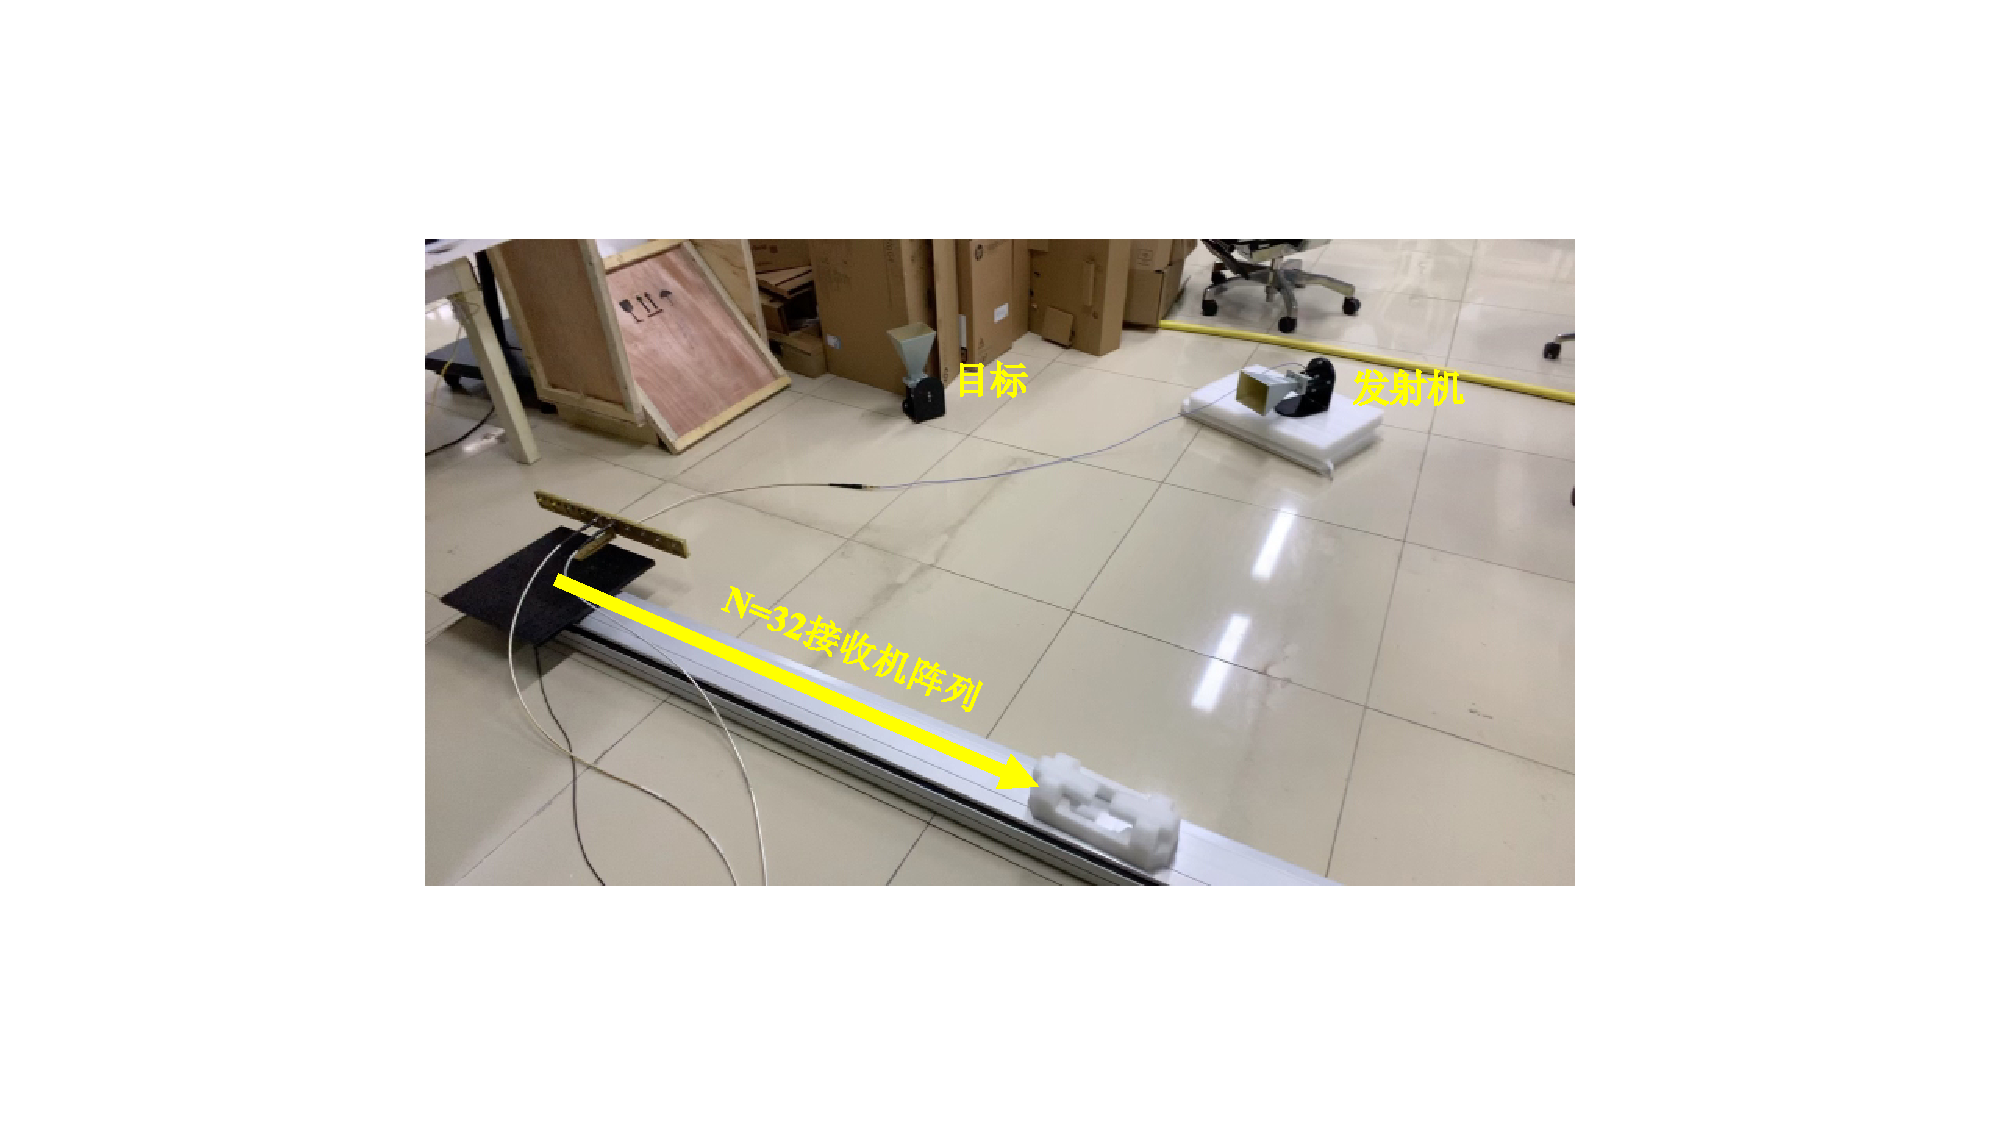
\includegraphics[width=.8\textwidth]{figures/exp/32.pdf}
  \caption{$N=32$实验场景}
  \label{32实验场景}
\end{figure}
\begin{figure}[H]
  \centering
  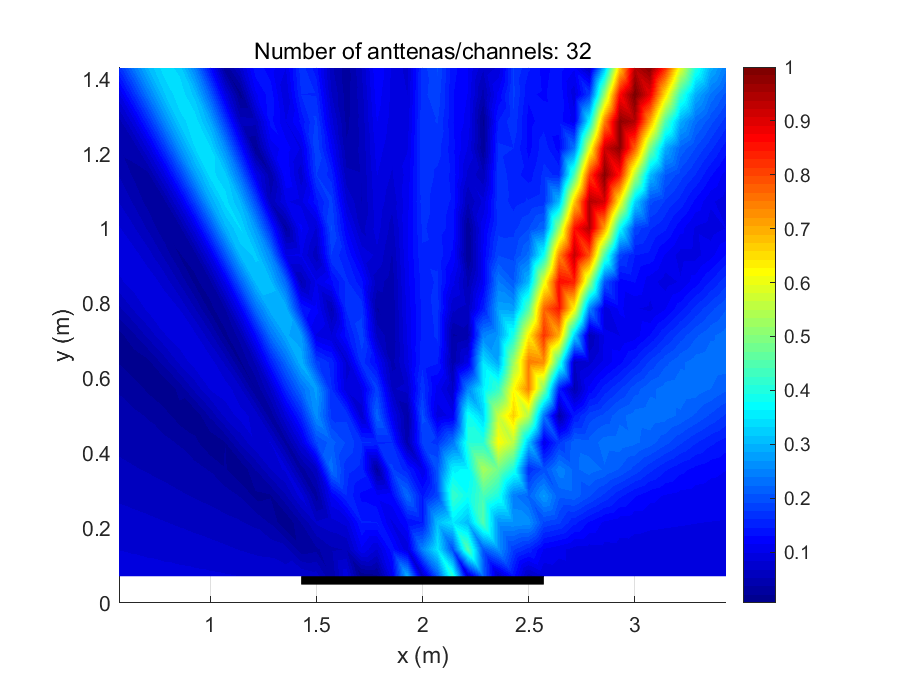
\includegraphics[width=.8\textwidth]{figures/exp/N32.eps}
  \caption{$N=32$对目标/信源成像结果}
  \label{32结果}
\end{figure}
\subsubsection{实验场景二:$N=64$对目标成像}
本小节对另一种成像场景进行了实测:不考虑对LOS径(信源)成像,而仅仅对目标成像。图~\ref{左},图~\ref{左结果}分别展示了利用数控轨道模拟的含64个阵元的接收机阵列对单个位于阵列左侧目标的成像场景及结果。
而图~\ref{右},图~\ref{右结果}分别展示了利用数控轨道模拟的含64个阵元的接收机阵列对单个位于阵列右侧目标的成像场景及结果。可以看出,在该场景下,本成像方案同样具有不错的效果。
\begin{figure}[H]
  \centering
  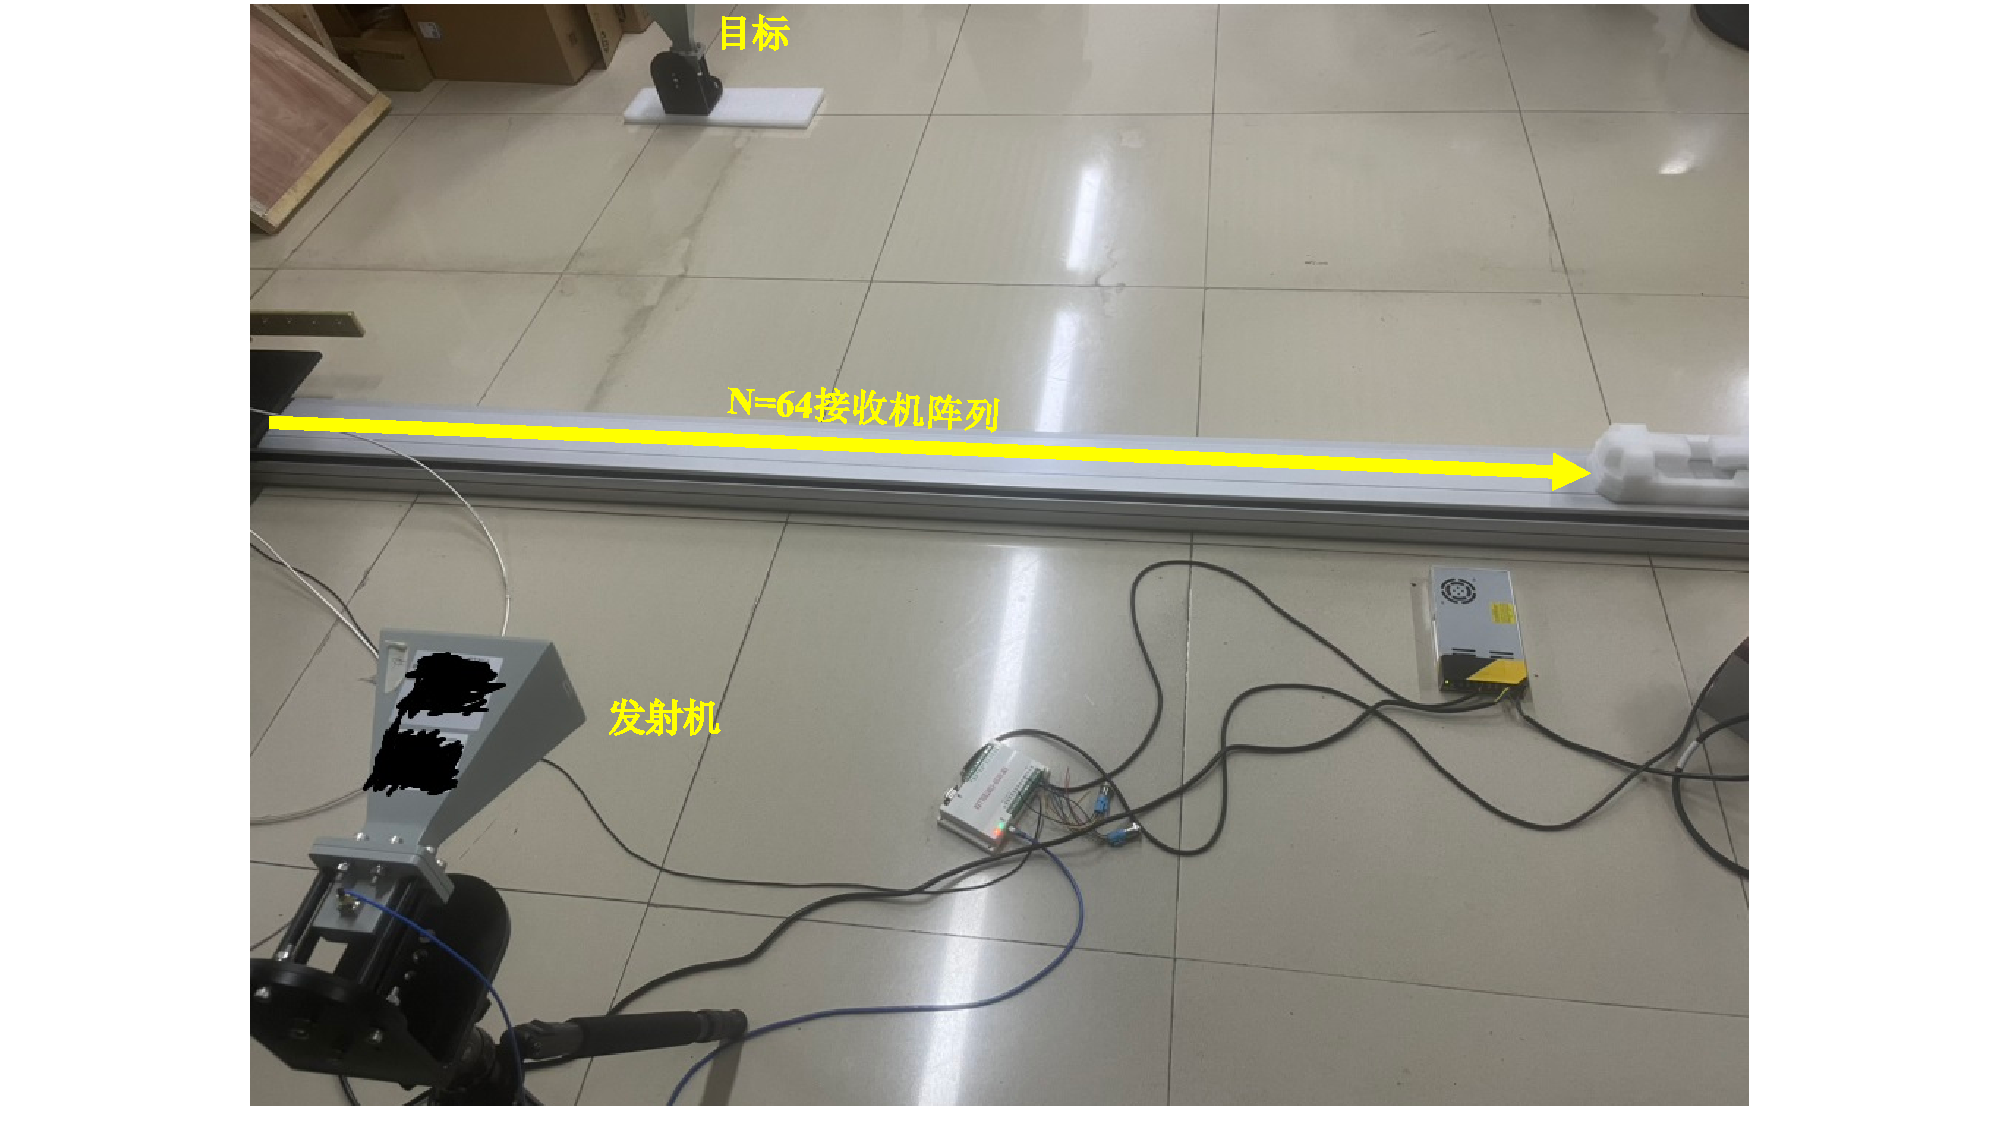
\includegraphics[width=.8\textwidth]{figures/exp/left.pdf}
  \caption{$N=64$对单目标成像场景(目标位于阵列左侧)}
  \label{左}
\end{figure}
\begin{figure}[H]
  \centering
  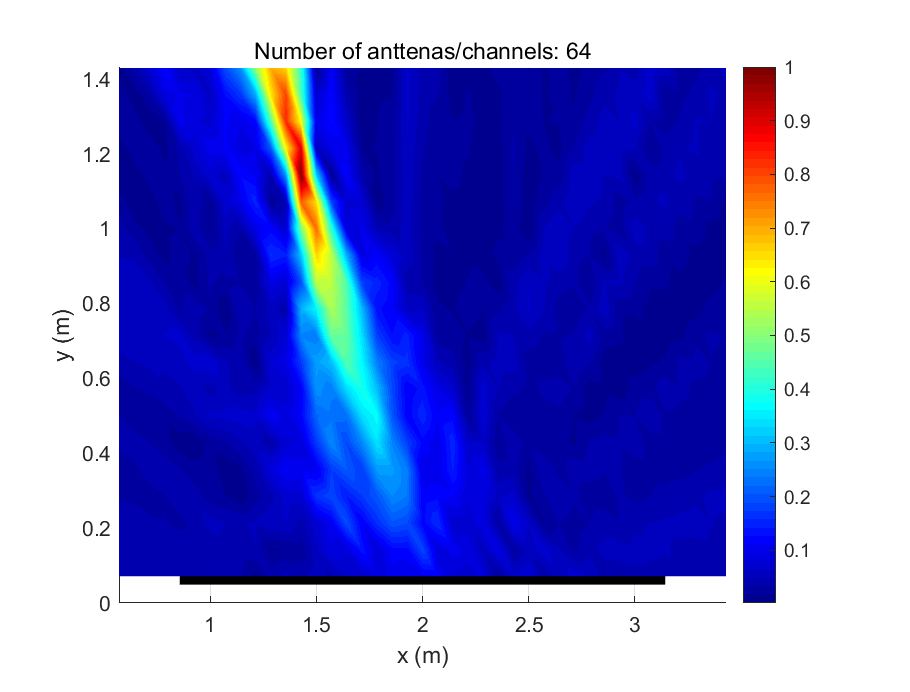
\includegraphics[width=.8\textwidth]{figures/exp/N64_left.eps}
  \caption{$N=64$对单目标成像结果(目标位于阵列左侧)}
  \label{左结果}
\end{figure}
\begin{figure}[H]
  \centering
  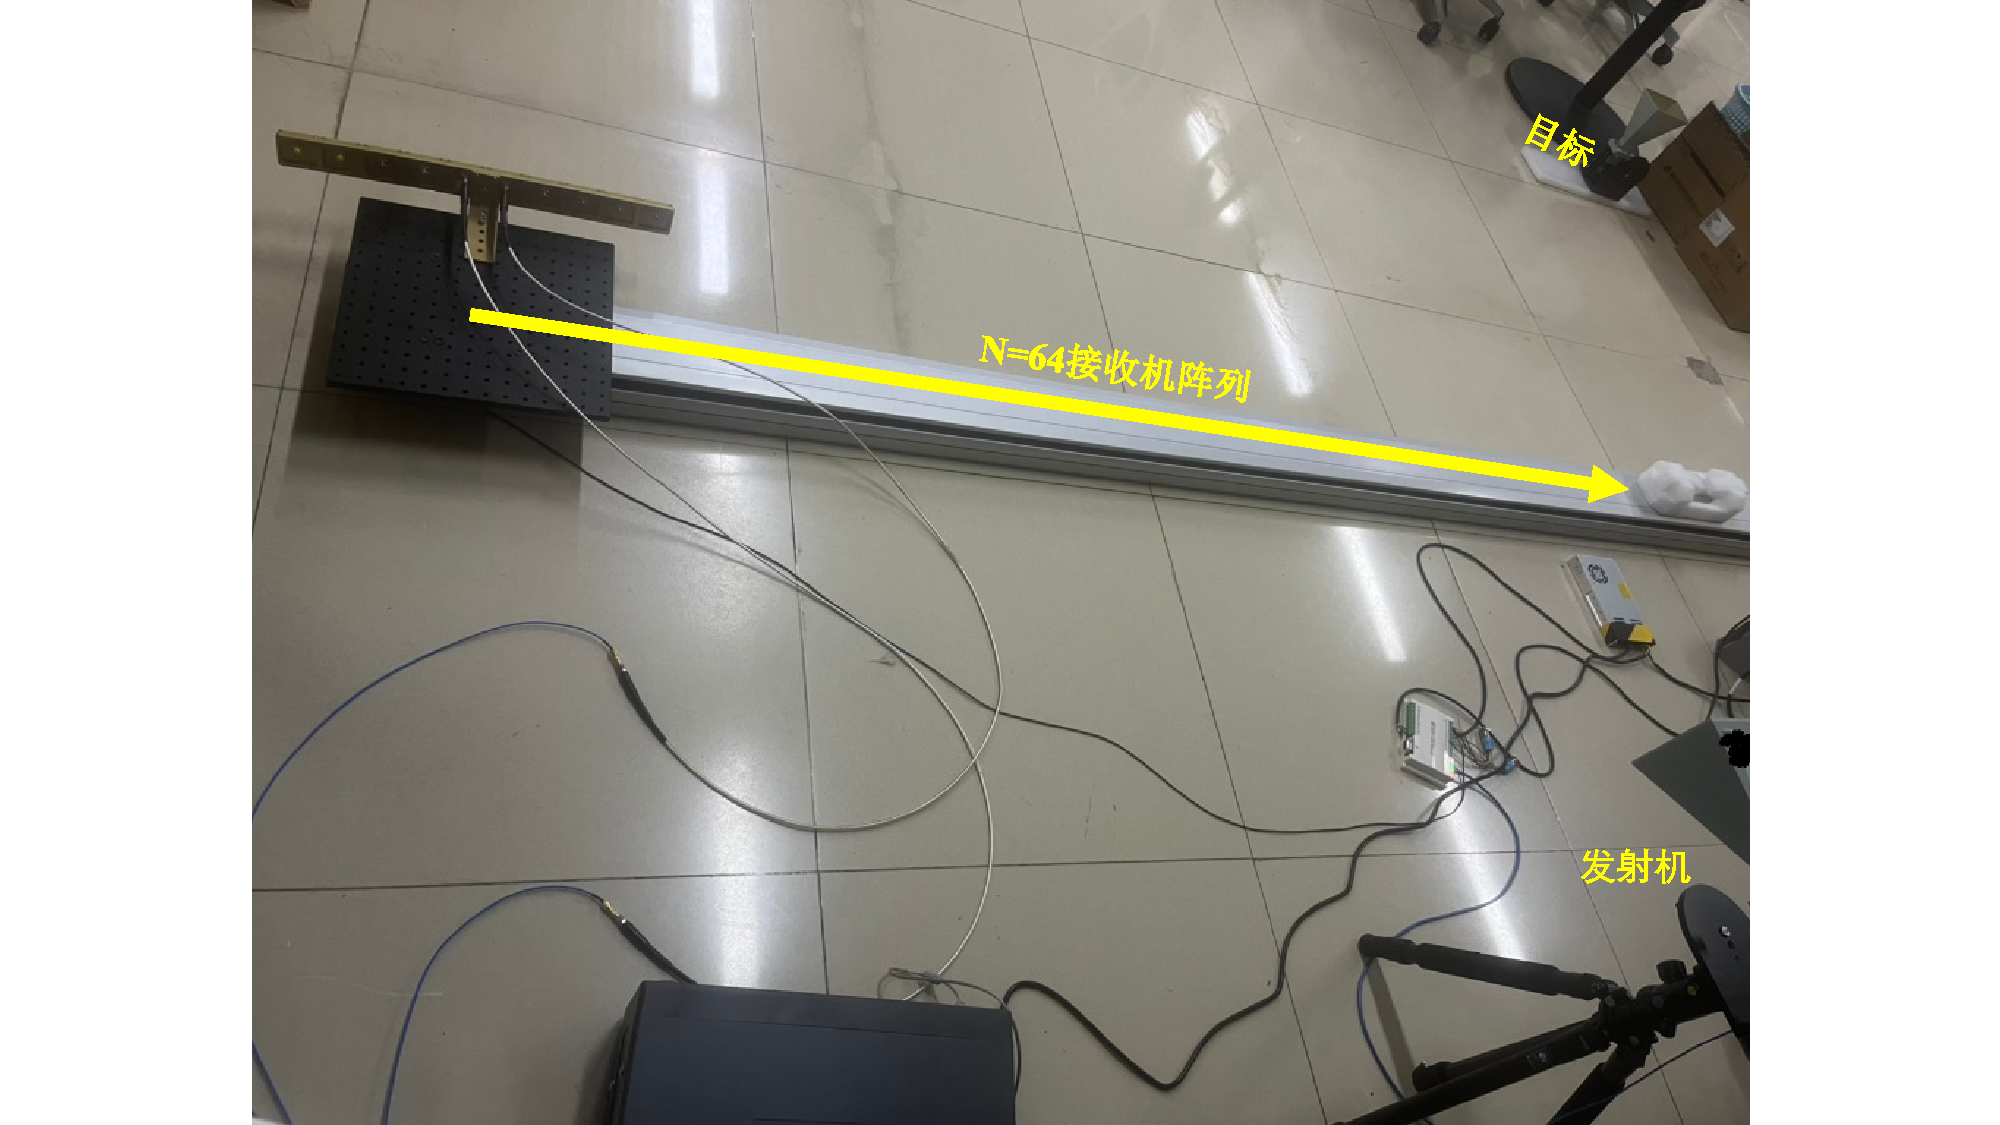
\includegraphics[width=.8\textwidth]{figures/exp/right.pdf}
  \caption{$N=64$对单目标成像场景(目标位于阵列右侧)}
  \label{右}
\end{figure}
\begin{figure}[H]
  \centering
  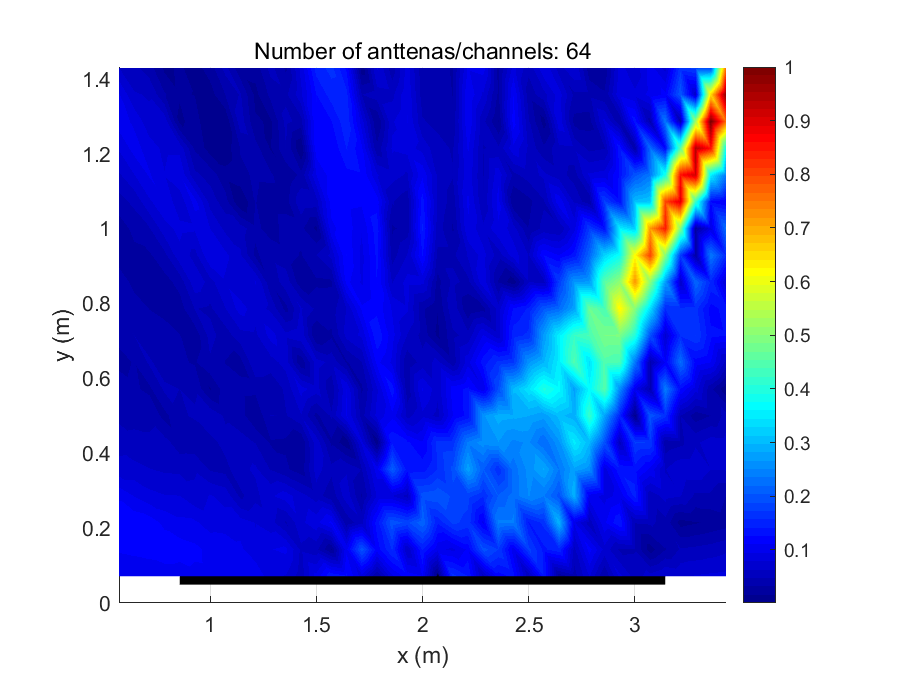
\includegraphics[width=.8\textwidth]{figures/exp/N64_right.eps}
  \caption{$N=64$对单目标成像场景(目标位于阵列右侧)}
  \label{右结果}
\end{figure}